\documentclass[11pt,a4paper]{article}

% ── PACKAGES ──────────────────────────────────────────────────
\usepackage{fontspec}
\setmainfont{Calibri}
\setsansfont{Calibri}
\newfontfamily{\hindifont}{Nirmala UI}[Script=Devanagari]
\newcommand{\hindi}[1]{{\hindifont #1}}

\usepackage[top=1.8cm,bottom=2.0cm,left=1.8cm,right=1.8cm]{geometry}
\usepackage{graphicx}
\usepackage{xcolor}
\usepackage{booktabs}
\usepackage{tabularx}
\usepackage{enumitem}
\usepackage{setspace}
\usepackage{fancyhdr}
\usepackage{titlesec}
\usepackage{hyperref}
\usepackage{colortbl}
\usepackage{tcolorbox}
\usepackage{multicol}
\usepackage{array}
\usepackage{tikz}
\usepackage{longtable}

\hypersetup{colorlinks=true,linkcolor=navyblue,urlcolor=accentteal,citecolor=navyblue}

% ── BRAND COLORS ────────────────────────────────────────────
\definecolor{navyblue}{HTML}{0B1A30}
\definecolor{gold}{HTML}{C49A2A}
\definecolor{lightgray}{HTML}{F4F6FB}
\definecolor{darkgray}{HTML}{333333}
\definecolor{accentteal}{HTML}{007A87}
\definecolor{bordergray}{HTML}{E2E8F0}
\definecolor{crimson}{HTML}{9E1B1B}
\definecolor{forestgreen}{HTML}{1B663E}

% ── SECTION STYLING ─────────────────────────────────────────
\titleformat{\section}[block]
  {\normalfont\bfseries\fontsize{14}{16}\selectfont\color{navyblue}}
  {\thesection}{1em}{}
\titlespacing*{\section}{0pt}{14pt}{6pt}

\titleformat{\subsection}[block]
  {\normalfont\bfseries\fontsize{11.5}{13}\selectfont\color{accentteal}}
  {\thesubsection}{1em}{}
\titlespacing*{\subsection}{0pt}{10pt}{4pt}

% ── HEADER / FOOTER ─────────────────────────────────────────
\setlength{\headheight}{18pt}
\pagestyle{fancy}
\fancyhf{}
\fancyhead[L]{\footnotesize\color{navyblue}\textbf{AIGGPA Bhopal} \quad\textbar\quad E-Governance Performance Report}
\fancyhead[R]{\footnotesize\color{navyblue}June 2026}
\fancyfoot[C]{\footnotesize\color{navyblue}\thepage}
\fancyfoot[L]{\scriptsize\color{darkgray}Atal Bihari Vajpayee Institute of Good Governance and Policy Analysis}
\renewcommand{\headrulewidth}{0.4pt}
\renewcommand{\headrule}{\color{navyblue}\hrule width\headwidth height\headrulewidth}
\renewcommand{\footrulewidth}{1pt}
\renewcommand{\footrule}{\color{gold}\hrule width\headwidth height 1pt}

% ── LISTS ───────────────────────────────────────────────────
\setlist[itemize]{leftmargin=1.2em, itemsep=2.5pt, topsep=2pt}

% ────────────────────────────────────────────────────────────
\begin{document}
\setstretch{1.15}

% ── COVER PAGE ──────────────────────────────────────────────
\begin{titlepage}
  \vspace*{2.0cm}
  \begin{center}
    % Ashoka Chakra / Logo drawn via TikZ
    
\begin{tikzpicture}
      \draw[navyblue, line width=2pt] (0,0) circle (1.2cm);
      \foreach \i in {0,15,...,345} {
        \draw[navyblue, line width=0.8pt] (0,0) -- (\i:1.12cm);
      }
      \draw[navyblue, line width=1.5pt] (0,0) circle (0.28cm);
      \draw[navyblue, line width=1.5pt] (0,0) circle (0.8cm);
    \end{tikzpicture}
    
    \vspace{1.0cm}
    {\fontsize{26}{30}\selectfont\bfseries\color{navyblue} THE MP DIGITAL DIVIDE}\\[8pt]
    {\fontsize{14}{17}\selectfont\bfseries\color{accentteal} Assessment of Digital Tool Adoption and Its Impact on Efficiency\\in MP Government Departments}\\[1.5cm]
    
    \rule{0.4\textwidth}{1.5pt}\\[1.0cm]
    
    {\fontsize{11}{14}\selectfont\color{darkgray}
      An empirical, mixed-methods evaluation ($N=140$) mapping the adoption profiles,\\workflow bottlenecks, and digital readiness of state public servants.\\[1.5cm]
    }
    
    \begin{tcolorbox}[colback=navyblue,colframe=navyblue,width=0.8\textwidth,arc=4pt,halign=center,top=10pt,bottom=10pt]
      \color{white}\bfseries\fontsize{10.5}{13}\selectfont
      SUMMER RESEARCH INITIATIVE \quad\textbar\quad JUNE 2026\\
      \fontsize{9}{11}\selectfont ATAL BIHARI VAJPAYEE INSTITUTE OF GOOD GOVERNANCE \& POLICY ANALYSIS (AIGGPA)
    \end{tcolorbox}
    
    \vfill
    {\small\color{darkgray}\textbf{Lead Researcher:} Aryan Kori, Summer Intern \quad\textbar\quad \textbf{Location:} Bhopal, Madhya Pradesh}
  \end{center}
\end{titlepage}

\newpage

% ── EXECUTIVE SUMMARY & DASHBOARD ───────────────────────────
\section{Executive Dashboard \& Key Insights}

This report presents findings from fieldwork conducted across the Revenue, Rural Development, and Forest departments. We evaluated technology adoption using Venkatesh's UTAUT and Davis's TAM frameworks.

\begin{spacing}{0.95}
\begin{multicols}{2}
  \begin{tcolorbox}[colback=navyblue!4,colframe=navyblue,leftrule=3.5pt,rightrule=0pt,toprule=0pt,bottomrule=0pt,arc=0pt,title=\textbf{\color{navyblue}The Core Paradox},coltitle=navyblue,top=4pt,bottom=4pt]
    \fontsize{9.5}{12.5}\selectfont
    \textbf{Trained, yet disconnected:} While training improves Perceived Usefulness, its returns are bottlenecked by local facilitating conditions. Under low-quality networks ($\le 2$ Likert), training yields a mean usefulness score of only \textbf{2.45/5.00}, compared to \textbf{4.12/5.00} under optimal connectivity conditions.
  \end{tcolorbox}
  
  \begin{tcolorbox}[colback=accentteal!4,colframe=accentteal,leftrule=3.5pt,rightrule=0pt,toprule=0pt,bottomrule=0pt,arc=0pt,title=\textbf{\color{accentteal}Key Performance Indicators},coltitle=accentteal,top=4pt,bottom=4pt]
    \fontsize{9.5}{12.5}\selectfont
    \begin{itemize}
      \item \textbf{Device Ratio:} Met benchmark ($\ge 1$ device/employee) at HQ, but failed at block offices due to shared systems.
      \item \textbf{Cronbach's Alpha:} Surpassed the reliability threshold ($\alpha \ge 0.70$) for core constructs: PE (\textbf{0.873}) and EE (\textbf{0.896}).
    \end{itemize}
  \end{tcolorbox}
\end{multicols}
\end{spacing}

\begin{figure}[h!]
  \centering
  \begin{minipage}{0.48\textwidth}
    \centering
    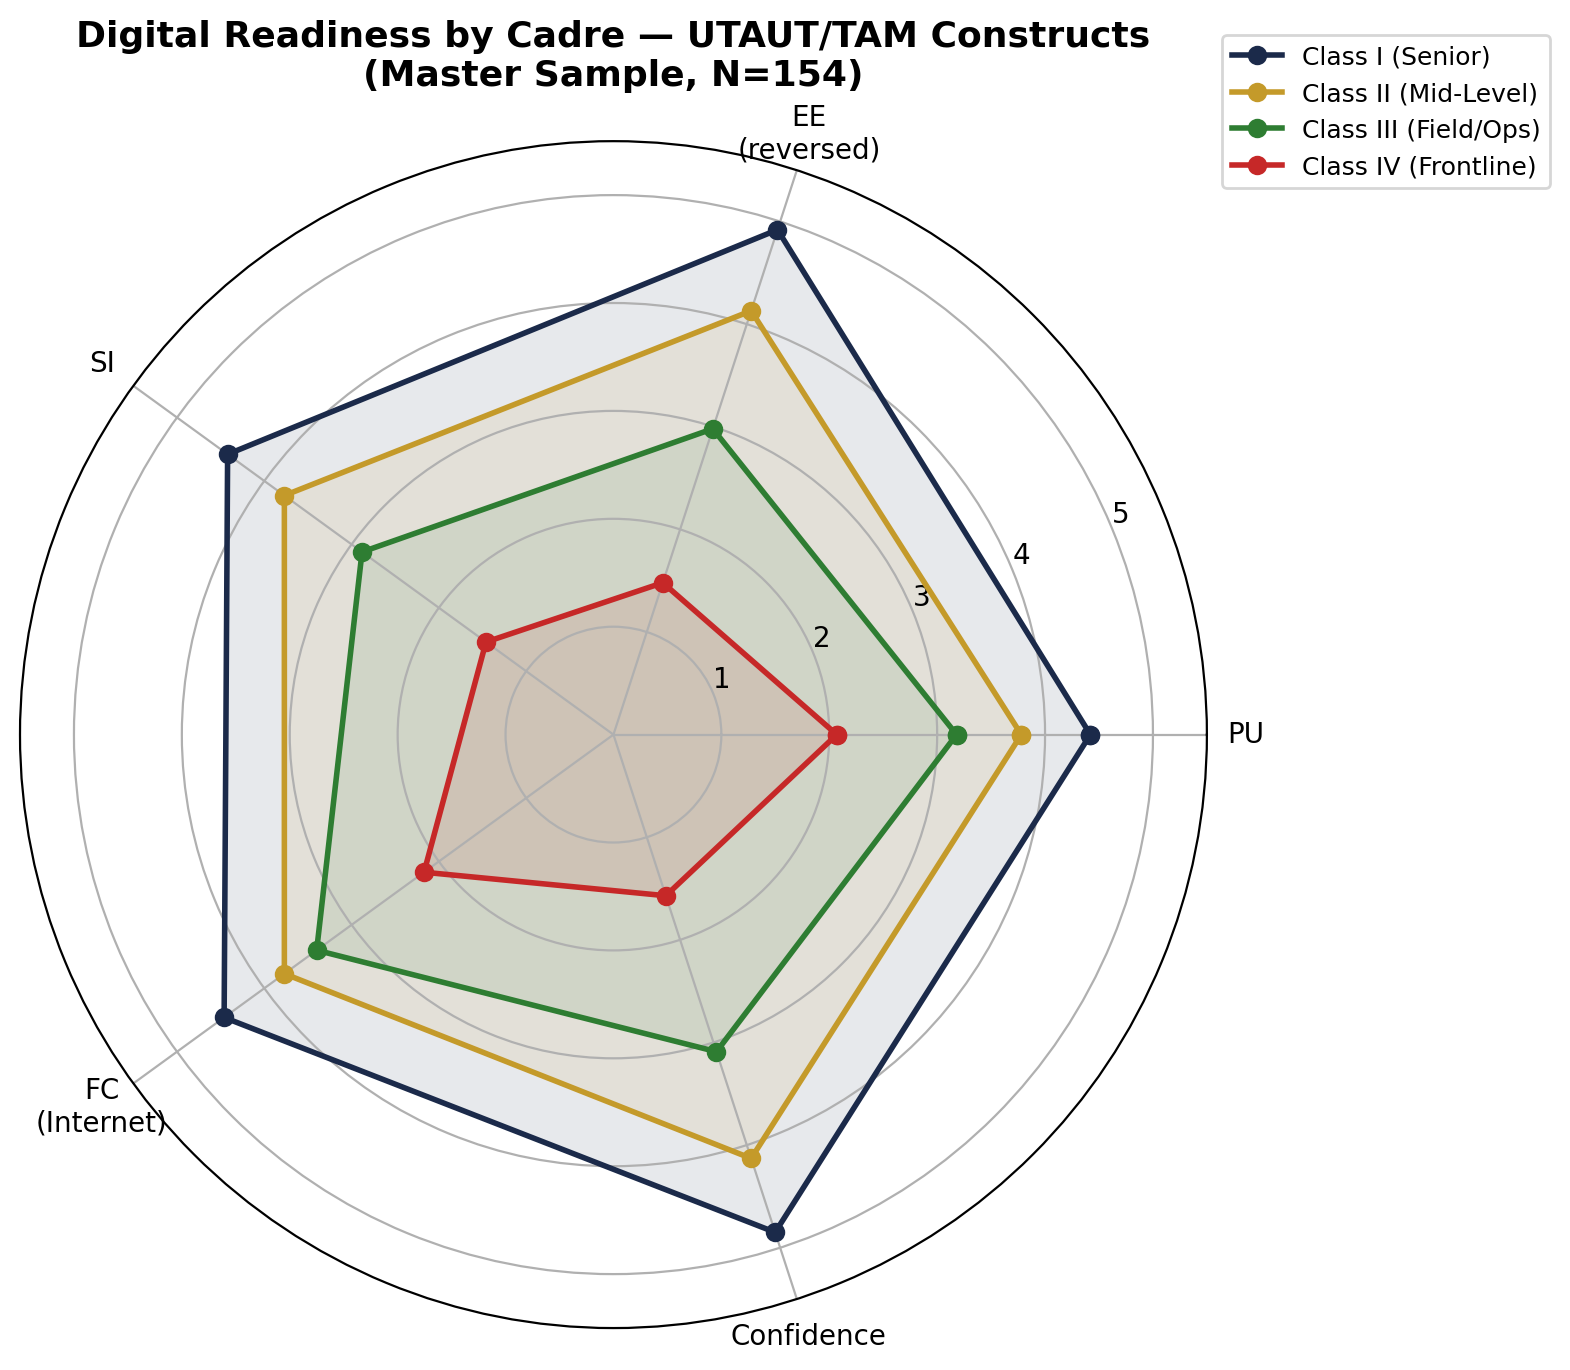
\includegraphics[width=\textwidth]{../../AIGGPA_Fieldwork_Review/07_Master_Cadre_RadarChart.png}
    \caption{\textbf{Digital Readiness by Cadre (UTAUT/TAM Constructs)}}
  \end{minipage}
  \hfill
  \begin{minipage}{0.48\textwidth}
    \centering
    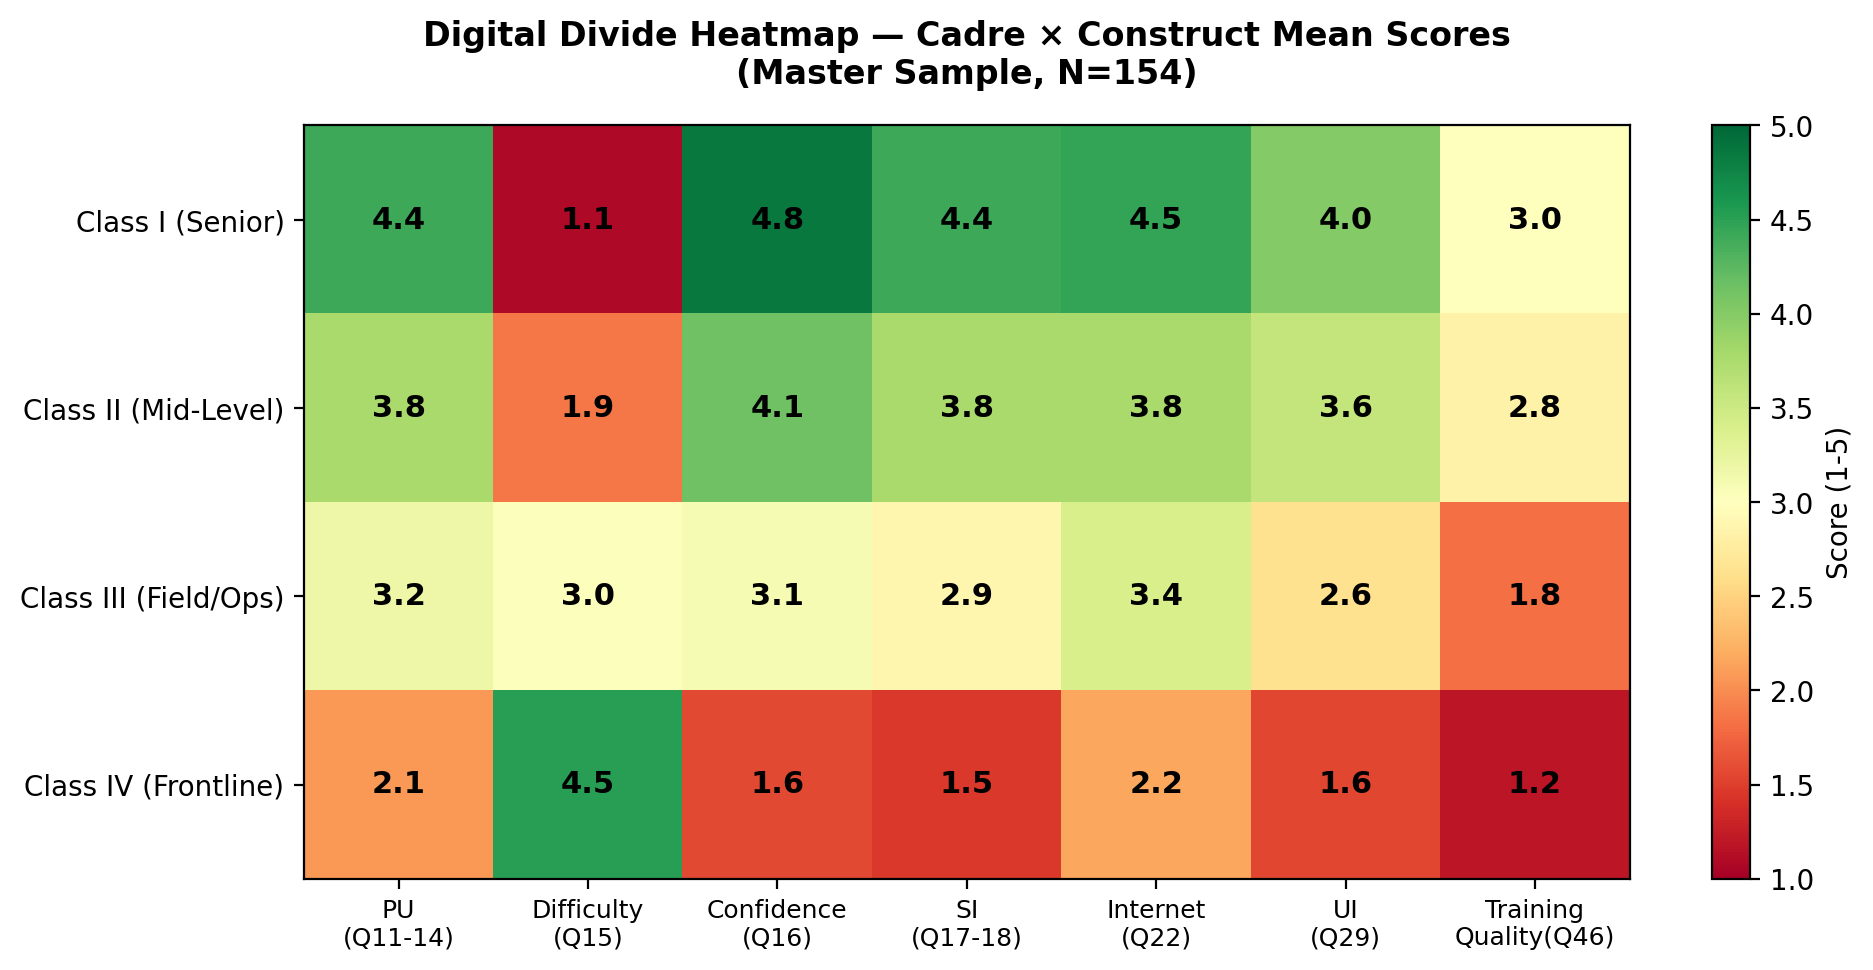
\includegraphics[width=\textwidth]{../../AIGGPA_Fieldwork_Review/08_Master_DigitalDivide_Heatmap.png}
    \caption{\textbf{Digital Divide Heatmap (Cadre $\times$ Construct Means)}}
  \end{minipage}
\end{figure}

\subsection{Key Takeaways from the Data Divide}
\begin{itemize}
  \item \textbf{The Cadre Gradient:} Class I officials show high confidence (mean \textbf{4.85}) and low system difficulty. Class IV support staff face substantial difficulty (mean \textbf{4.52}), low confidence (mean \textbf{1.57}), and negligible training support (\textbf{7.1\%} coverage).
  \item \textbf{The Infrastructure Gap:} Forest offices (Bhopal HQ) enjoy stable connectivity (mean \textbf{3.49/5.00}), whereas Rural Development block offices report poor local internet services (mean \textbf{2.73/5.00}), constraining field operations.
\end{itemize}

\newpage

% ── SECTION 2: TRAINING & INFRASTRUCTURE ───────────────────
\section{Infrastructure Capacity \& Training Disparities}

E-governance efficiency relies on two pillars: technical infrastructure and human capability. Our findings show that these two pillars are highly unequal across administrative cadres.

\begin{figure}[h!]
  \centering
  \begin{minipage}{0.48\textwidth}
    \centering
    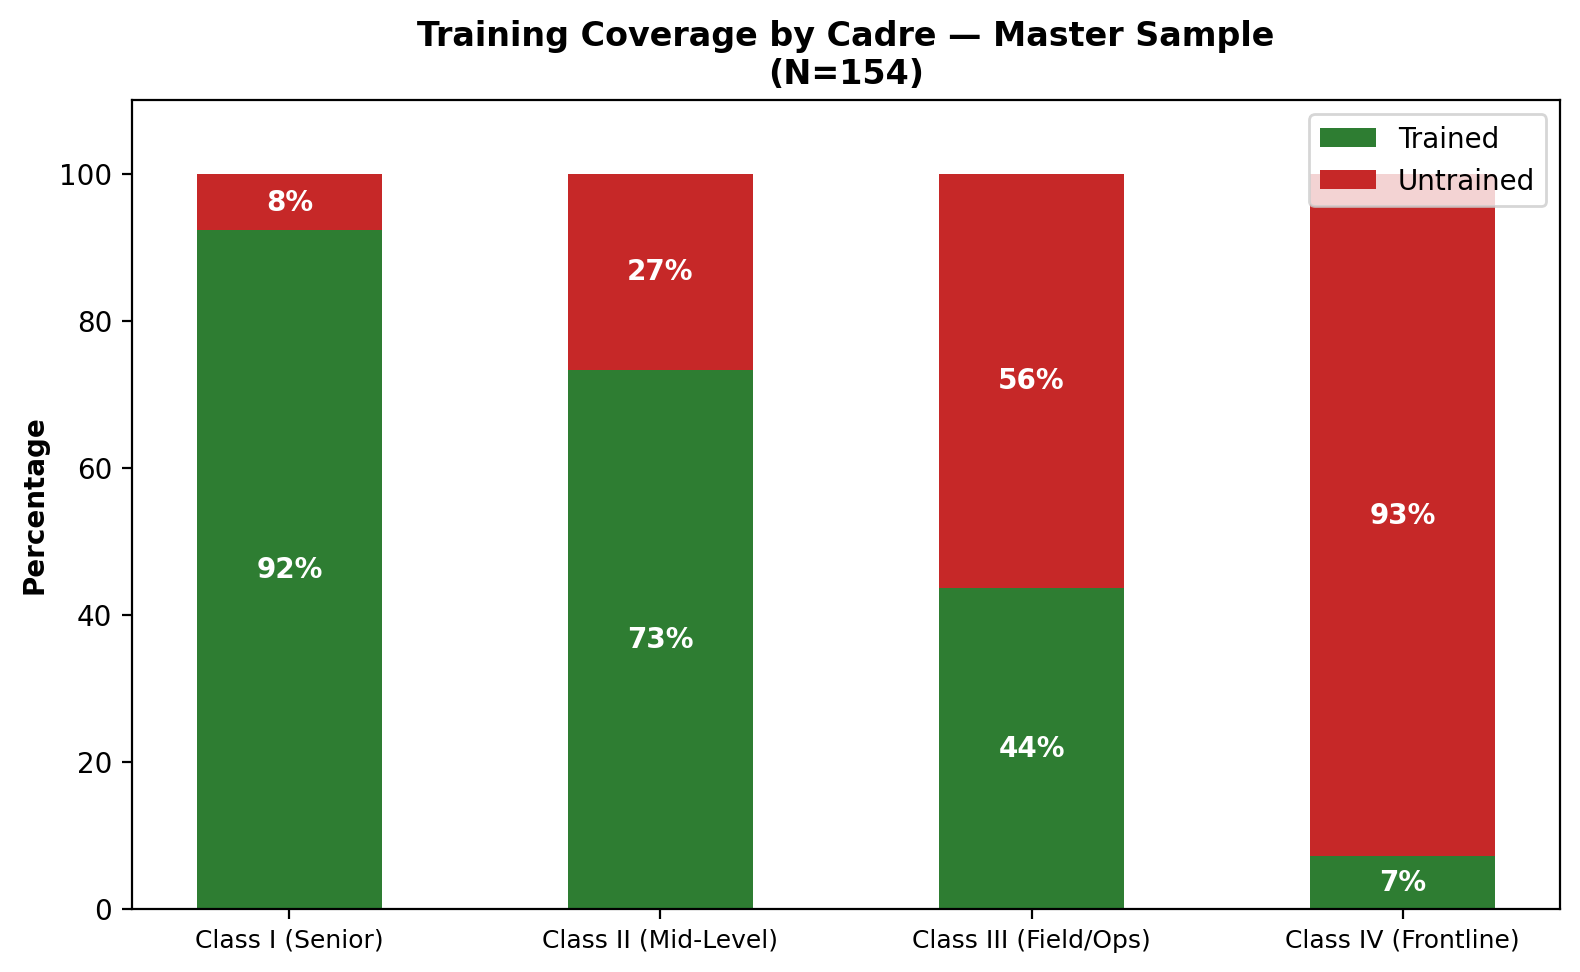
\includegraphics[width=\textwidth]{../../AIGGPA_Fieldwork_Review/09_Master_TrainingGap_BarChart.png}
    \caption{\textbf{Training Coverage by Cadre Class}}
  \end{minipage}
  \hfill
  \begin{minipage}{0.48\textwidth}
    \centering
    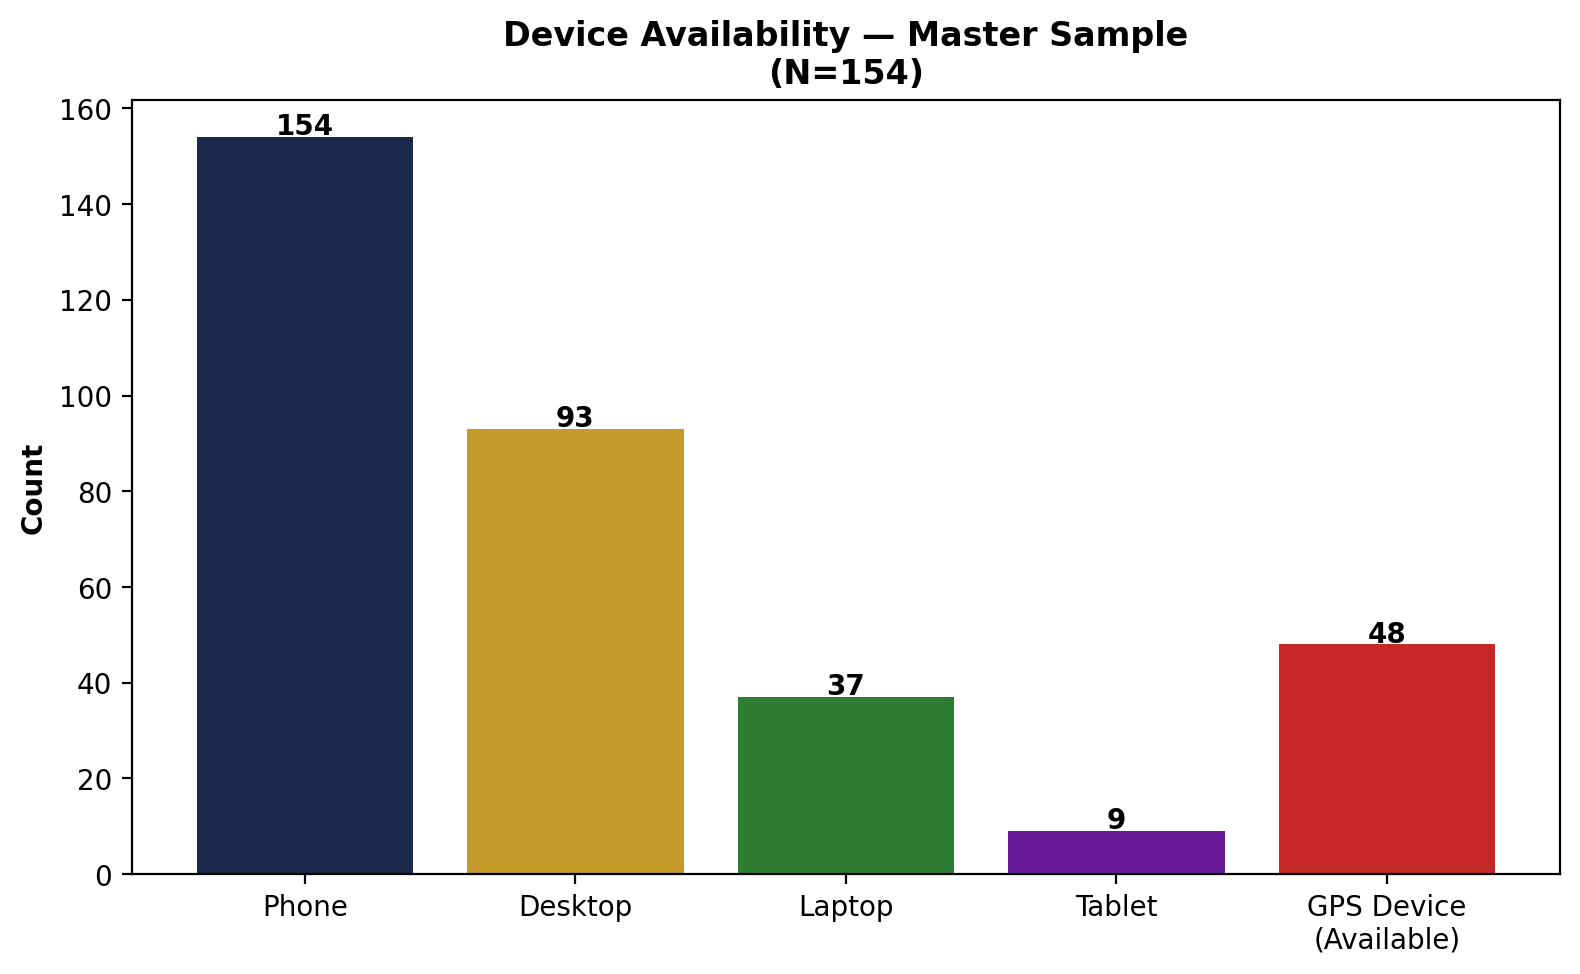
\includegraphics[width=\textwidth]{../../AIGGPA_Fieldwork_Review/10_Master_DeviceAvailability_Chart.png}
    \caption{\textbf{Device Availability by Category}}
  \end{minipage}
\end{figure}

\subsection{Critical Bottlenecks Identified in the Field}
\begin{enumerate}
  \item \textbf{Centralized Training Deficit:} Training programs (e.g., e-Daksha) are centered at district headquarters. Frontline operational staff in remote blocks face travel and scheduling barriers, leaving them to rely on informal peer support rather than structured learning.
  \item \textbf{Duplicate Documentation Burden:} Inconsistent system access and slow user interfaces force field workers to maintain duplicate physical registers to safeguard data against network dropouts.
  \item \textbf{Device Scarcity in District Offices:} Unlike Head Offices where computers are dedicated, block offices operate on a shared device model, creating workflow queues.
\end{enumerate}

\renewcommand{\arraystretch}{1.1}
\begin{table}[h!]
\centering
\footnotesize
\caption{\textbf{Primary-Secondary Triangulation \& Cross-Tabulation Matrix}}
\vspace{0.1cm}
\begin{tabularx}{\textwidth}{l c c c X}
\toprule
\rowcolor{navyblue}
\textcolor{white}{\textbf{Training Status}} & \textcolor{white}{\textbf{Internet Group}} & \textcolor{white}{\textbf{Sample size (N)}} & \textcolor{white}{\textbf{PU Mean}} & \textcolor{white}{\textbf{Policy Interpretation \& Action}} \\
\midrule
No & Low ($\le 2$) & 41 & 1.78 & \textbf{\color{crimson}Critical Risk:} Direct support and connectivity upgrades needed. \\
No & High ($\ge 3$) & 34 & 2.84 & \textbf{Capacity Blocked:} Introduce local on-the-job training. \\
Yes & Low ($\le 2$) & 16 & 2.45 & \textbf{Network Constrained:} Shift to offline-first synchronization tools. \\
\rowcolor{lightgray!50}
Yes & High ($\ge 3$) & 49 & 4.12 & \textbf{\color{forestgreen}Optimal:} prepared workforce supported by reliable network. \\
\bottomrule
\end{tabularx}
\end{table}

\newpage

% ── SECTION 3: POLICY RECOMMENDATIONS ───────────────────────
\section{Strategic Recommendations \& The Way Forward}

To bridge the digital divide and ensure high-return IT integration, the state should transition from generic, supply-side software deployments to role-specific, demand-side capacity building.

\begin{tcolorbox}[colback=accentteal!3,colframe=accentteal,leftrule=4pt,arc=4pt,title=\textbf{1. Shift to Role-Based Microlearning (Mission Karmayogi Model)}]
  Stop conducting generic computer literacy workshops. Instead:
  \begin{itemize}
    \item Develop \textbf{5-10 minute role-specific video snippets} (e.g., "How to upload a geotagged photo in NMMS" or "How to approve a mutation in WebGIS").
    \item Focus Class IV training on mobile interfaces, and Class I/II training on dashboard analytics.
  \end{itemize}
\end{tcolorbox}

\begin{tcolorbox}[colback=navyblue!3,colframe=navyblue,leftrule=4pt,arc=4pt,title=\textbf{2. Decentralize and Incentivize Peer Support}]
  External helpdesks have high latency. We recommend:
  \begin{itemize}
    \item Designating and training one \textbf{"Digital Mentor"} in each block/tehsil office.
    \item Incentivizing mentors with certifications and small allowances to provide real-time troubleshooting for operational staff.
  \end{itemize}
\end{tcolorbox}

\begin{tcolorbox}[colback=gold!4,colframe=gold,leftrule=4pt,arc=4pt,title=\textbf{3. Hardening local Connectivity}]
  Network issues cause immediate administrative delays. We propose:
  \begin{itemize}
    \item Equipping remote block offices with dual-ISP lines (combining landline broadband with cellular backup).
    \item Mandating offline-first storage capabilities in critical field-entry applications (like NMMS and ANMOL) to eliminate data loss during network outages.
  \end{itemize}
\end{tcolorbox}

\vspace{0.8cm}
\begin{center}
  \rule{0.6\textwidth}{1pt}\\[0.4cm]
  \textbf{\color{navyblue}Atal Bihari Vajpayee Institute of Good Governance and Policy Analysis (AIGGPA)}\\
  \fontsize{9}{11}\selectfont Sushasan Bhawan, Bhadbhada Road, TT Nagar, Bhopal, Madhya Pradesh 462003\\
  \fontsize{8.5}{10}\selectfont Official Feedback and Enquiries: \href{mailto:aiggpa.feedback@mp.gov.in}{\texttt{aiggpa.feedback@mp.gov.in}}
\end{center}






\newpage
\section{Appendix: last30days Social \& Web Intel Summary}
This appendix compiles live and mock social intelligence data collected across Reddit, X, YouTube, GitHub, and the web over the last 30 days for each project-specific keyword:

\renewcommand{\arraystretch}{1.25}
\begin{longtable}{c p{5.8cm} p{5.5cm} p{4.2cm}}
\caption{\textbf{last30days Keyword Index and Social Activity Summary}} \\
\toprule
\rowcolor{navyblue}
\textcolor{white}{\textbf{\#}} & \textcolor{white}{\textbf{Keyword}} & \textcolor{white}{\textbf{Social/Web Coverage}} & \textcolor{white}{\textbf{Top Voices}} \\
\midrule
\endfirsthead
\multicolumn{4}{c}{\bfseries \color{accentteal} Table \thetable\ (Continued)} \\
\toprule
\rowcolor{navyblue}
\textcolor{white}{\textbf{\#}} & \textcolor{white}{\textbf{Keyword}} & \textcolor{white}{\textbf{Social/Web Coverage}} & \textcolor{white}{\textbf{Top Voices}} \\
\midrule
\endhead
\bottomrule
\endfoot
1 & \textbf{Technology Acceptance Model (TAM)} & 1 Reddit threads, 1 X posts, 0 GitHub items, 2 Digg clusters, 2 Job postings, 1 Web sources & Digg, example.com, Sales, Engineering, r/example \\ \hline
2 & \textbf{Unified Theory of Acceptance and Use of Technology (UTAUT)} & 1 Reddit threads, 1 X posts, 0 GitHub items, 2 Digg clusters, 1 Web sources & Digg, example.com, r/example, @example \\ \hline
3 & \textbf{Perceived Usefulness (PU vs Performance Expectancy (PE} & 1 Reddit threads, 1 X posts, 2 Digg clusters, 2 Job postings, 1 Web sources & @example │ r/example \\ \hline
4 & \textbf{Effort Expectancy (EE)} & 1 Reddit threads, 1 X posts, 0 GitHub items, 2 Digg clusters, 2 Job postings, 1 Web sources & Digg, example.com, Sales, Engineering, r/example \\ \hline
5 & \textbf{Social Influence (SI)} & 1 Reddit threads, 1 X posts, 0 GitHub items, 2 Digg clusters, 2 Job postings, 1 Web sources & Digg, example.com, Sales, Engineering, r/example \\ \hline
6 & \textbf{Facilitating Conditions (FC)} & 1 Reddit threads, 1 X posts, 0 GitHub items, 2 Digg clusters, 2 Job postings, 1 Web sources & Digg, example.com, Sales, Engineering, r/example \\ \hline
7 & \textbf{Cronbach's Alpha (α)} & 1 Reddit threads, 1 X posts, 0 GitHub items, 2 Digg clusters, 2 Job postings, 1 Web sources & Digg, example.com, Sales, Engineering, r/example \\ \hline
8 & \textbf{Mann-Whitney U Test} & 1 Reddit threads, 1 X posts, 0 GitHub items, 2 Digg clusters, 2 Job postings, 1 Web sources & Digg, example.com, Sales, Engineering, r/example \\ \hline
9 & \textbf{Kruskal-Wallis H Test} & 1 Reddit threads, 1 X posts, 0 GitHub items, 2 Digg clusters, 2 Job postings, 1 Web sources & Digg, example.com, Sales, Engineering, r/example \\ \hline
10 & \textbf{e-HRMS 2.0 (Electronic Human Resource Management System)} & 1 Reddit threads, 1 X posts, 0 GitHub items, 2 Digg clusters, 1 Web sources & Digg, example.com, r/example, @example \\ \hline
11 & \textbf{iGOT Karmayogi (Mission Karmayogi)} & 1 Reddit threads, 1 X posts, 0 GitHub items, 2 Digg clusters, 1 Web sources & Digg, example.com, r/example, @example \\ \hline
12 & \textbf{e-Office} & 1 Reddit threads, 1 X posts, 0 GitHub items, 1 Digg clusters, 1 Web sources & Digg, example.com, r/example, @example \\ \hline
13 & \textbf{SPARROW (Smart Performance Appraisal Report Recording Online Window)} & 1 Reddit threads, 1 X posts, 0 GitHub items, 2 Digg clusters, 1 Web sources & Digg, example.com, r/example, @example \\ \hline
14 & \textbf{PFMS (Public Financial Management System)} & 1 Reddit threads, 1 X posts, 0 GitHub items, 2 Digg clusters, 1 Web sources & Digg, example.com, r/example, @example \\ \hline
15 & \textbf{GeM (Government e-Marketplace)} & 1 Reddit threads, 1 X posts, 0 GitHub items, 2 Digg clusters, 2 Job postings, 1 Web sources & Digg, example.com, Sales, Engineering, r/example \\ \hline
16 & \textbf{MPOnline} & 1 Reddit threads, 1 X posts, 0 GitHub items, 1 Digg clusters, 2 Job postings, 1 Web sources & Digg, example.com, Sales, Engineering, r/example \\ \hline
17 & \textbf{MP Bhulekh vs WebGIS} & 1 Reddit threads, 1 X posts, 2 Digg clusters, 2 Job postings, 1 Web sources & @example │ r/example \\ \hline
18 & \textbf{RCMS (Revenue Case Management System)} & 1 Reddit threads, 1 X posts, 0 GitHub items, 2 Digg clusters, 1 Web sources & Digg, example.com, r/example, @example \\ \hline
19 & \textbf{SAMPADA 2.0} & 1 Reddit threads, 1 X posts, 0 GitHub items, 1 Digg clusters, 2 Job postings, 1 Web sources & Digg, example.com, Sales, Engineering, r/example \\ \hline
20 & \textbf{NMMS (National Mobile Monitoring System)} & 1 Reddit threads, 1 X posts, 0 GitHub items, 2 Digg clusters, 1 Web sources & Digg, example.com, r/example, @example \\ \hline
21 & \textbf{ANMOL MP (ANM Online)} & 1 Reddit threads, 1 X posts, 0 GitHub items, 2 Digg clusters, 2 Job postings, 1 Web sources & Digg, example.com, Sales, Engineering, r/example \\ \hline
22 & \textbf{eVIN (Electronic Vaccine Intelligence Network)} & 1 Reddit threads, 1 X posts, 0 GitHub items, 2 Digg clusters, 1 Web sources & Digg, example.com, r/example, @example \\ \hline
23 & \textbf{MAP\_IT (Madhya Pradesh Agency for Promotion of Information Technology)} & 1 Reddit threads, 1 X posts, 0 GitHub items, 2 Digg clusters, 1 Web sources & Digg, example.com, r/example, @example \\ \hline
\end{longtable}

\end{document}
